\documentclass[conference]{IEEEtran}

\usepackage[utf8]{inputenc}
\usepackage[T1]{fontenc}
\usepackage{mathptmx}
\usepackage[spanish,es-tabla,es-noshorthands,es-nolayout]{babel}
\addto\captionsspanish{\renewcommand{\figurename}{Fig.}\renewcommand{\refname}{Referencias}}
\usepackage{amsmath}
\usepackage{graphicx}
\usepackage{booktabs}
\usepackage{array}
\usepackage{textcomp}
\usepackage{cite}
\usepackage{url}
\usepackage{microtype}
\usepackage{makecell}

\newcommand{\ohmm}{\ensuremath{\Omega\!\cdot\!\mathrm{m}}}
\newcommand{\rhoa}{\ensuremath{\rho_a}}
\graphicspath{{figs/}}
\hyphenation{Ben Fellah Guerrara}

\begin{document}
\renewcommand{\IEEEkeywordsname}{Palabras clave}

\title{Anomal\'ias de resistividad compatibles con procesos k\'arsticos en Dayat Ben Fellah (Argelia): confiabilidad y modelo conceptual}

\author{\IEEEauthorblockN{Ian A. Sandoval-Valderr\'abano}
\IEEEauthorblockA{\textit{Colegio de Geof\'isica, Facultad de Ingenier\'ia}\\
\textit{Benem\'erita Universidad Aut\'onoma de Puebla}\\
Puebla, M\'exico}}

\maketitle

\begin{abstract}
Se estudiaron diez perfiles de tomograf\'ia de resistividad el\'ectrica (ERT, arreglo Wenner) medidos en la depresi\'on k\'arstica de Dayat Ben Fellah, en el sur de Argelia. Se ubicaron los perfiles en UTM 31N y sobre una imagen satelital, se dibujaron pseudosecciones y modelos con escala y unidades, y se invirtieron los diez con tres niveles de suavizado. La inversi\'on se compar\'o con los modelos de Res2DInv disponibles de BF1, BF2 y BF7. El RMS de Res2DInv fue 1.64, 4.92 y 5.43\,\%, pero los datos de BF1 casi no cambian (factor 1.9) y en BF2 el 77\,\% de los bloques tiene incertidumbre mayor a 15\,\%. De las 14 anomal\'ias candidatas de BF1 y BF2, solo 3 se reproducen bien con la inversi\'on propia, 5 en parte y 6 no; ninguna de BF1 se reproduce. En cuatro perfiles (BF4, BF5, BF6 y BF10) el ajuste es pobre y no se interpretan. En los otros seis, la inversi\'on propia marca seis candidatas prioritarias. Pueden deberse a huecos, a rellenos de arcilla o humedad, o a fracturas, pero ninguna se presenta como cavidad comprobada. Se propone un modelo conceptual, pruebas para verificarlas y las limitaciones del estudio.
\end{abstract}

\begin{IEEEkeywords}
tomograf\'ia de resistividad el\'ectrica, karst, cavidades, fracturas, Res2DInv, incertidumbre, Argelia
\end{IEEEkeywords}

\section{Introducci\'on}
En zonas \'aridas, el agua de lluvia con di\'oxido de carbono disuelve carbonatos y yeso. As\'i se abren huecos que pueden hundirse y da\~nar obras y acu\'iferos. La ERT mide qu\'e tanto se opone el terreno al paso de la corriente (resistividad). Se usa mucho para buscar estos huecos porque es r\'apida y no da\~na el terreno \cite{melouah2016,coskun2012,elkhammari2007}. Pero una misma anomal\'ia puede tener varias causas: un hueco con aire, roca compacta o material seco dan resistividad alta; un hueco relleno de arcilla, una lente de arcilla o arena h\'umeda dan resistividad baja.

Este informe responde la pregunta gu\'ia de la Actividad~3: \emph{\textquestiondown qu\'e anomal\'ias de resistividad pueden deberse a disoluci\'on, fracturas o cavidades, y qu\'e informaci\'on falta para evaluar su importancia ambiental y geot\'ecnica?} Con los datos de Dayat Ben Fellah \cite{melouah2016} se hizo lo siguiente: (i) ubicar los perfiles, (ii) dibujar pseudosecciones y modelos con escalas y unidades, (iii) medir qu\'e tan confiable es cada modelo sin depender solo del RMS, (iv) invertir los diez perfiles y comparar el resultado con Res2DInv, (v) armar un modelo conceptual del subsuelo y (vi) proponer c\'omo verificarlo. Ninguna anomal\'ia se presenta como cavidad comprobada y el RMS no es el \'unico criterio de confiabilidad.

\section{Datos y \'area de estudio}
Dayat Ben Fellah es una depresi\'on de unos 1.96\,km por 1.33\,km, en la regi\'on de Guerrara (Ghard\"a\"ia), cerca de 32°43$'$\,N y 4°37$'$\,E. El art\'iculo la explica como un hundimiento k\'arstico en carbonatos del Eoceno, guiado por fracturas con direcciones N\,50--70° y N\,150--170°. Tambi\'en describe huecos de tama\~no m\'etrico, sin conexi\'on entre s\'i y en parte rellenos de sedimentos \cite{melouah2016}. Dentro de la depresi\'on, la arenisca est\'a a menos de 10\,m y tiene 80 a 140\,\ohmm; el aluvi\'on tiene 20 a 70\,\ohmm. En una secci\'on del sitio, el aluvi\'on tiene m\'as de 35\,\% de carbonatos y una resistencia a la compresi\'on de 19\,bar (unos 1.9\,MPa) \cite{melouah2016}.

Se dispone de diez perfiles (archivos \texttt{.txt} en formato Res2DInv, arreglo Wenner, con separaciones $a$ de 5 a 40\,m; en BF7, de 2.5 a 12.5\,m). Tambi\'en se dispone de los modelos de Res2DInv de BF1, BF2 y BF7 (archivos \texttt{.INV}) y las coordenadas de inicio y fin de cada perfil (\texttt{CORDON2.xls}). En esos tres perfiles, los datos de los \texttt{.txt} y los \texttt{.INV} son iguales. BF1 termina a 1\,m del inicio de BF2, as\'i que juntos forman una sola l\'inea de 350\,m. El encabezado de BF8 dice 116 datos, pero el archivo trae 117; se usaron los 117.

La Tabla~\ref{tab:perfiles} resume los perfiles y el ajuste de las inversiones (se explican m\'as adelante). La Fig.~\ref{fig:mapa} los ubica sobre la imagen satelital: todos quedan dentro o junto al fondo plano de la depresi\'on. BF1 y BF2 lo cruzan de norte a sur. BF7 queda en el borde de una estructura circular de unos 150\,m, cerca del centro. La imagen no dice qu\'e es, as\'i que no se interpreta; conviene revisarla en campo.

\subsection{Geolog\'ia regional}
La Fig.~\ref{fig:geo} resume la geolog\'ia que da el art\'iculo \cite{melouah2016}, y la ubicaci\'on de la zona sale de su mapa geol\'ogico regional (su Fig.~1a). En superficie hay aluviones del Cuaternario (QT), areniscas del Mio-plioceno (MP), Plioceno continental (PC) y, al oeste, Cret\'acico superior (CS). Con la cuadr\'icula UTM de ese mapa, la zona de los perfiles cae sobre MP, junto a una franja de QT que sigue el drenaje al oeste-suroeste. Es una lectura aproximada, con error de unos 100\,m. En profundidad, el art\'iculo menciona caliza con fosfatos del Eoceno, carbonatos marinos del Senoniano (acu\'ifero de unos 275\,m), calizas, arcillas y yesos alternados hasta unos 650\,m, y el Continental Intercalar. La ERT solo ve la parte alta del Cuaternario y del Mio-plioceno.

\begin{figure}[!t]
\centering
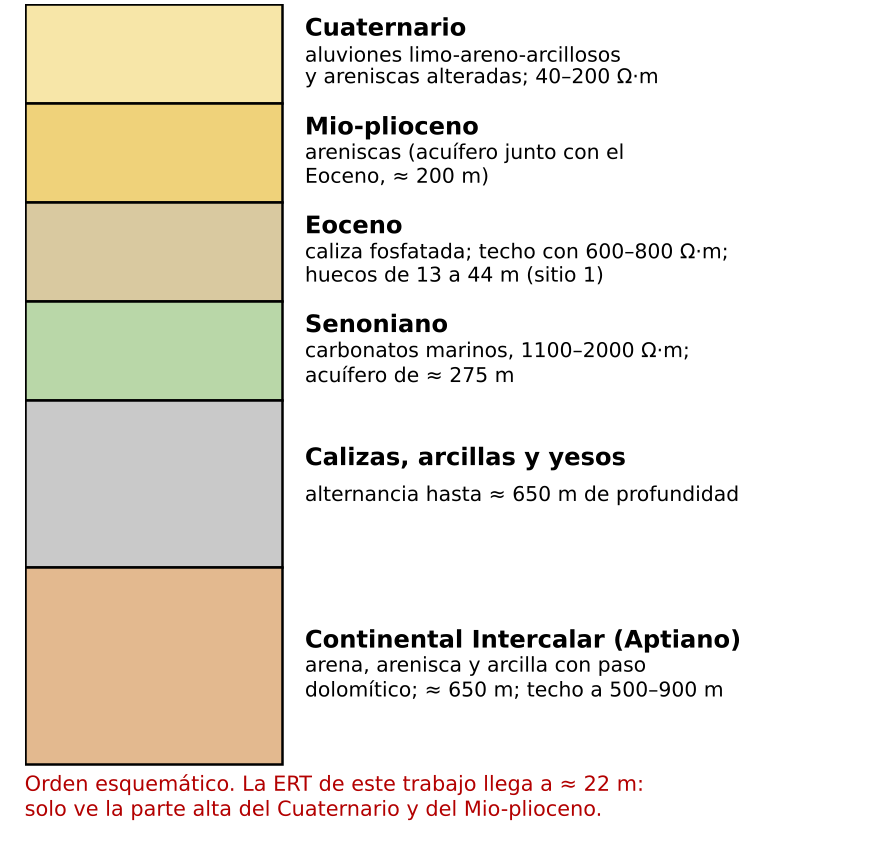
\includegraphics[width=0.92\columnwidth]{f7_columna.png}
\caption{Columna estratigr\'afica esquem\'atica, sin escala, hecha con los datos del texto de Melouah y Zeddouri \cite{melouah2016}.}
\label{fig:geo}
\end{figure}

\begin{table*}[!t]
\caption{Perfiles: longitud declarada y calculada con las coordenadas, azimut, n\'umero de datos y rango de $\rho_a$. Ajuste: RMS (\%) de Res2DInv (solo BF1, BF2, BF7) y de la inversi\'on propia con suavizado d\'ebil / base / fuerte; porcentaje de datos con error $>10$\,\% en el modelo base; y si el ajuste es aceptable (RMS base $\le 8$\,\% y menos de 10\,\% de datos con error $>10$\,\%).}
\label{tab:perfiles}
\centering\footnotesize
\setlength{\tabcolsep}{5pt}
\begin{tabular}{lccccccccc}
\toprule
Perfil & Dec. (m) & Coord. (m) & Azimut (°) & Datos & \rhoa{} (\ohmm) & RMS Res2DInv & RMS propio & Err.\,$>10$\,\% & Aceptable \\
\midrule
BF1 & 170 & 165 & 186 & 80 & 61--114 & 1.64 & 2.0 / 2.6 / 3.1 & 0 & sí \\
BF2 & 180 & 183 & 190 & 122 & 87--202 & 4.92 & 4.6 / 5.0 / 5.5 & 4 & sí \\
BF3 & 110 & 111 & 184 & 53 & 9--46 & -- & 4.0 / 6.2 / 9.0 & 9 & sí \\
BF4 & 180 & 180 & 157 & 118 & 13--56 & -- & 7.6 / 10.6 / 12.3 & 34 & no \\
BF5 & 175 & 171 & 331 & 116 & 16--74 & -- & 9.1 / 9.3 / 13.8 & 22 & no \\
BF6 & 175 & 184 & 80 & 116 & 24--87 & -- & 12.8 / 13.8 / 15.4 & 43 & no \\
BF7 & 45 & 35 & 63 & 35 & 29--170 & 5.43 & 3.0 / 4.5 / 5.9 & 3 & sí \\
BF8 & 175 & 168 & 65 & 117 & 20--89 & -- & 5.0 / 5.8 / 6.8 & 8 & sí \\
BF9 & 170 & 167 & 343 & 112 & 42--102 & -- & 2.6 / 3.7 / 4.4 & 1 & sí \\
BF10 & 175 & 162 & 105 & 117 & 8--44 & -- & 6.1 / 7.9 / 10.9 & 18 & no \\
\bottomrule
\end{tabular}
\end{table*}

\begin{figure}[!t]
\centering
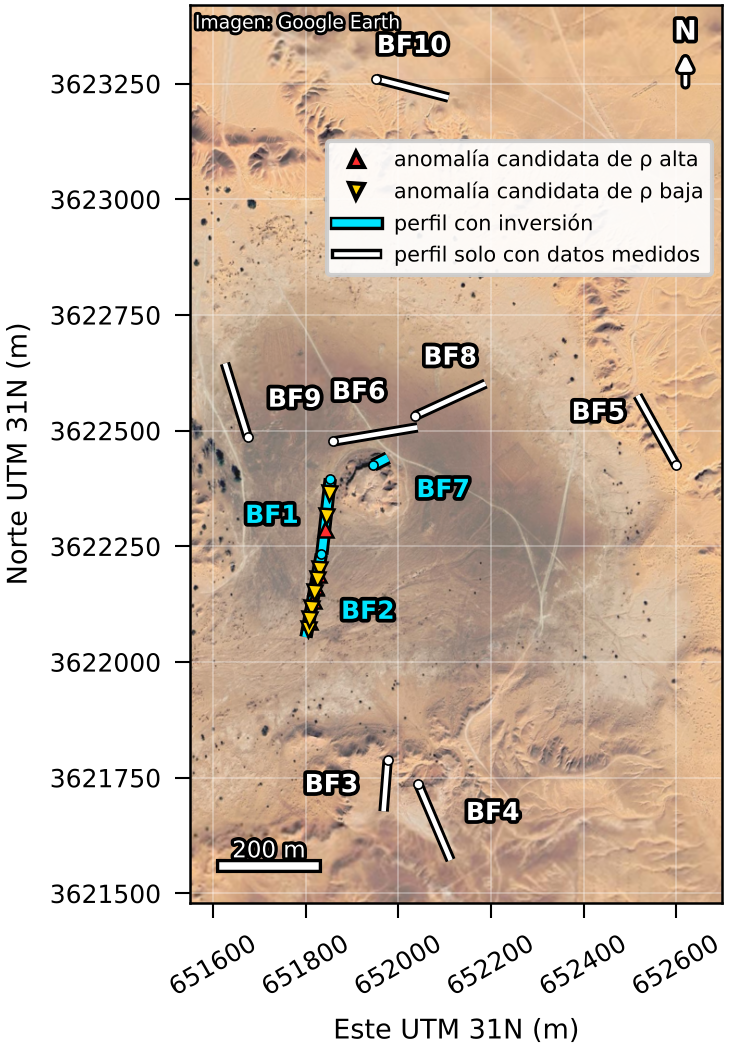
\includegraphics[width=0.94\columnwidth]{f1_mapa.png}
\caption{Perfiles ubicados en UTM zona 31N (WGS84) con \texttt{CORDON2.xls}, sobre una imagen satelital de Google Earth. Los tri\'angulos son las anomal\'ias candidatas de BF1 y BF2 (Tabla~\ref{tab:cand}); BF1 y BF2 forman una l\'inea continua. La imagen se ubic\'o con un punto conocido y la barra de escala (error de unos 15\,m).}
\label{fig:mapa}
\end{figure}

\section{M\'etodos}
\subsection{Ubicaci\'on de los perfiles}
Las coordenadas en grados, minutos y segundos se pasaron a UTM 31N con \texttt{pyproj}. El resultado coincide con las columnas Este y Norte de la hoja \texttt{Feuil3}, con una diferencia m\'axima de 0.0005\,m en los nueve perfiles que las traen. BF1 no ten\'ia valores UTM y se calcul\'o.

La imagen de fondo de la Fig.~\ref{fig:mapa} son dos capturas de Google Earth, vistas desde arriba y con el norte arriba. La primera se ubic\'o con un punto conocido (32°43$'$48.0$''$\,N, 4°37$'$12.0$''$\,E) y su barra de escala (300\,m). La segunda se aline\'o con la primera con 813 puntos comunes (error de 0.3 p\'ixeles). El norte de la malla UTM est\'a girado 0.88° respecto del de la imagen, y se corrigi\'o con \texttt{pyproj}. La incertidumbre es de unos 15\,m.

Los grados vienen redondeados a 0.1$''$ (unos 3\,m) y se supone una l\'inea recta, as\'i que un punto del perfil tiene incertidumbre de 3 a 10\,m. La longitud calculada difiere de la declarada hasta 7\,\% en nueve perfiles y 23\,\% en BF7 (Tabla~\ref{tab:perfiles}).

\subsection{Pseudosecciones y modelos}
Para el arreglo Wenner, la pseudoprofundidad es
\begin{equation}
z_p = 0.519\,a, \label{eq:zp}
\end{equation}
con $a$ la separaci\'on entre electrodos \cite{edwards1977}. La posici\'on horizontal es el punto medio del arreglo. Las pseudosecciones se dibujaron con los datos medidos y con los calculados por Res2DInv en la \'ultima iteraci\'on.

Los modelos de BF1, BF2 y BF7 son los calculados con Res2DInv 3.53g. Este programa hace una inversi\'on de Gauss--Newton que busca un modelo suave, con elementos finitos, topograf\'ia y el logaritmo de $\rho_a$ \cite{loke1996}. Esos tres modelos no se recalcularon. De los archivos se ley\'o, para cada bloque, su resistividad, sensibilidad e incertidumbre (\%), y el RMS de cada iteraci\'on.

\subsection{Inversi\'on propia}
Los diez perfiles se invirtieron con un c\'odigo en Python. El c\'odigo resuelve el problema directo en 2.5D con elementos finitos y topograf\'ia, y busca un modelo suave con Gauss--Newton, en logaritmo de $\rho$ y de $\rho_a$, parecido en idea al de \cite{loke1996}. El ancho de los bloques es la separaci\'on de electrodos de cada perfil y hay 12 capas, de 1.0 m de espesor arriba a 5.0 m abajo (a escala de la separaci\'on). Se supuso un error de 3\,\% en cada dato y no se borr\'o ning\'un dato. Se calcul\'o con tres niveles de suavizado (d\'ebil, base y fuerte; amortiguamiento inicial de 6, 20 y 60, que baja 30\,\% en cada una de las 12 iteraciones). El RMS propio es el error relativo cuadr\'atico medio (\%); se parece al de Res2DInv, pero no es id\'entico. Un perfil se interpreta solo si el RMS del modelo base es $\le 8$\,\% y menos de 10\,\% de los datos tiene error $>10$\,\%.

\subsection{Confiabilidad m\'as all\'a del RMS}
Para los modelos de Res2DInv se usaron seis indicadores (el RMS es solo el primero): (1) el RMS inicial, el final y su cambio en la \'ultima iteraci\'on; (2) el error de cada dato, $\varepsilon=\ln(\rho_{med}/\rho_{calc})$, por nivel $a$ y por posici\'on; (3) si el contraste de una anomal\'ia se mantiene entre iteraciones; (4) la sensibilidad y la incertidumbre de cada bloque; (5) el contraste de los datos medidos frente al del modelo; y (6) si el resultado concuerda con el art\'iculo y con la geometr\'ia de la medici\'on.

\subsection{Anomal\'ias candidatas}
En cada capa de bloques se tom\'o como fondo la mediana de $\log_{10}\rho$ y se calcul\'o
\begin{equation}
\Delta(x,z)=\log_{10}\rho(x,z)-\mathrm{mediana}_{capa}\,(\log_{10}\rho). \label{eq:delta}
\end{equation}
Una regi\'on conectada con $|\Delta|\ge 0.30$ (factor 2 en resistividad) y \'area m\'inima de 15\,m$^2$ (ajustada al tama\~no del bloque) se marc\'o como candidata de resistividad alta (H) o baja (L). A cada una se le dio un \'indice de soporte $S$ de 0 a 4, con un punto por cada criterio que cumple: incertidumbre media $\le 20$\,\%; sensibilidad media $\ge 0.4$; contraste ya presente en la iteraci\'on 4 ($\ge$ factor 1.3); y $\rho_a$ medida en su zona con el mismo signo ($\ge$ 12\,\% respecto de la mediana de su nivel). Los umbrales son de este trabajo, no de Res2DInv. $S$ sirve para ordenar la prioridad de verificaci\'on; no mide la probabilidad de que haya una cavidad. En los modelos propios se us\'o el mismo criterio de contraste y un $S$ adaptado, porque no hay incertidumbre por bloque: (1) la anomal\'ia aparece con el mismo signo en los modelos d\'ebil y fuerte ($|\Delta|\ge 0.15$); (2) la cobertura media (suma de la sensibilidad) es mayor que la mediana del perfil; (3) en el modelo fuerte el contraste es $\ge$ factor 1.3; y (4) igual que antes, para $\rho_a$. Una candidata propia es \emph{prioritaria} si $S\ge 3$, cumple (2), tiene $\ge 30$\,m$^2$, no est\'a limitada a la primera capa (el dato m\'as somero tiene $z_p=2.6$\,m) y su perfil tiene ajuste aceptable. Para comparar con Res2DInv, cada una de sus candidatas se busca sobre el mismo recuadro del modelo propio y se calcula el factor de contraste con signo. Si es $\ge 1.5$ se dice que \emph{se reproduce}; entre 1.2 y 1.5, \emph{en parte}; si es menor o de signo opuesto, \emph{no}. Estos umbrales tambi\'en son de este trabajo.

\section{Resultados}
\subsection{Datos medidos}
La Fig.~\ref{fig:pseudo} muestra BF1, BF2 y BF7. En BF1, $\rho_a$ var\'ia de 61 a 114\,\ohmm, un factor de solo 1.9, con un m\'aximo en $z_p\approx 10$\,m y $x\approx 80$\,m. En BF2 va de 87 a 202\,\ohmm{} y baja con la profundidad (mediana de 164\,\ohmm{} con $a=5$\,m y de 92\,\ohmm{} con $a=40$\,m). BF7 est\'a en una ladera de unos 18° y tiene 35 datos.

La Fig.~\ref{fig:otros} muestra los otros siete perfiles, que no traen modelo de Res2DInv. BF3 y BF10, que seg\'un \texttt{CORDON2.xls} est\'an en las alturas de la periferia, son los m\'as conductores, con medianas de 14 a 36\,\ohmm. En los siete, $\rho_a$ crece con $a$ (por ejemplo en BF8, de 30 a 78\,\ohmm). Es compatible con una cobertura blanda sobre un fondo m\'as resistivo.

\begin{figure*}[!t]
\centering
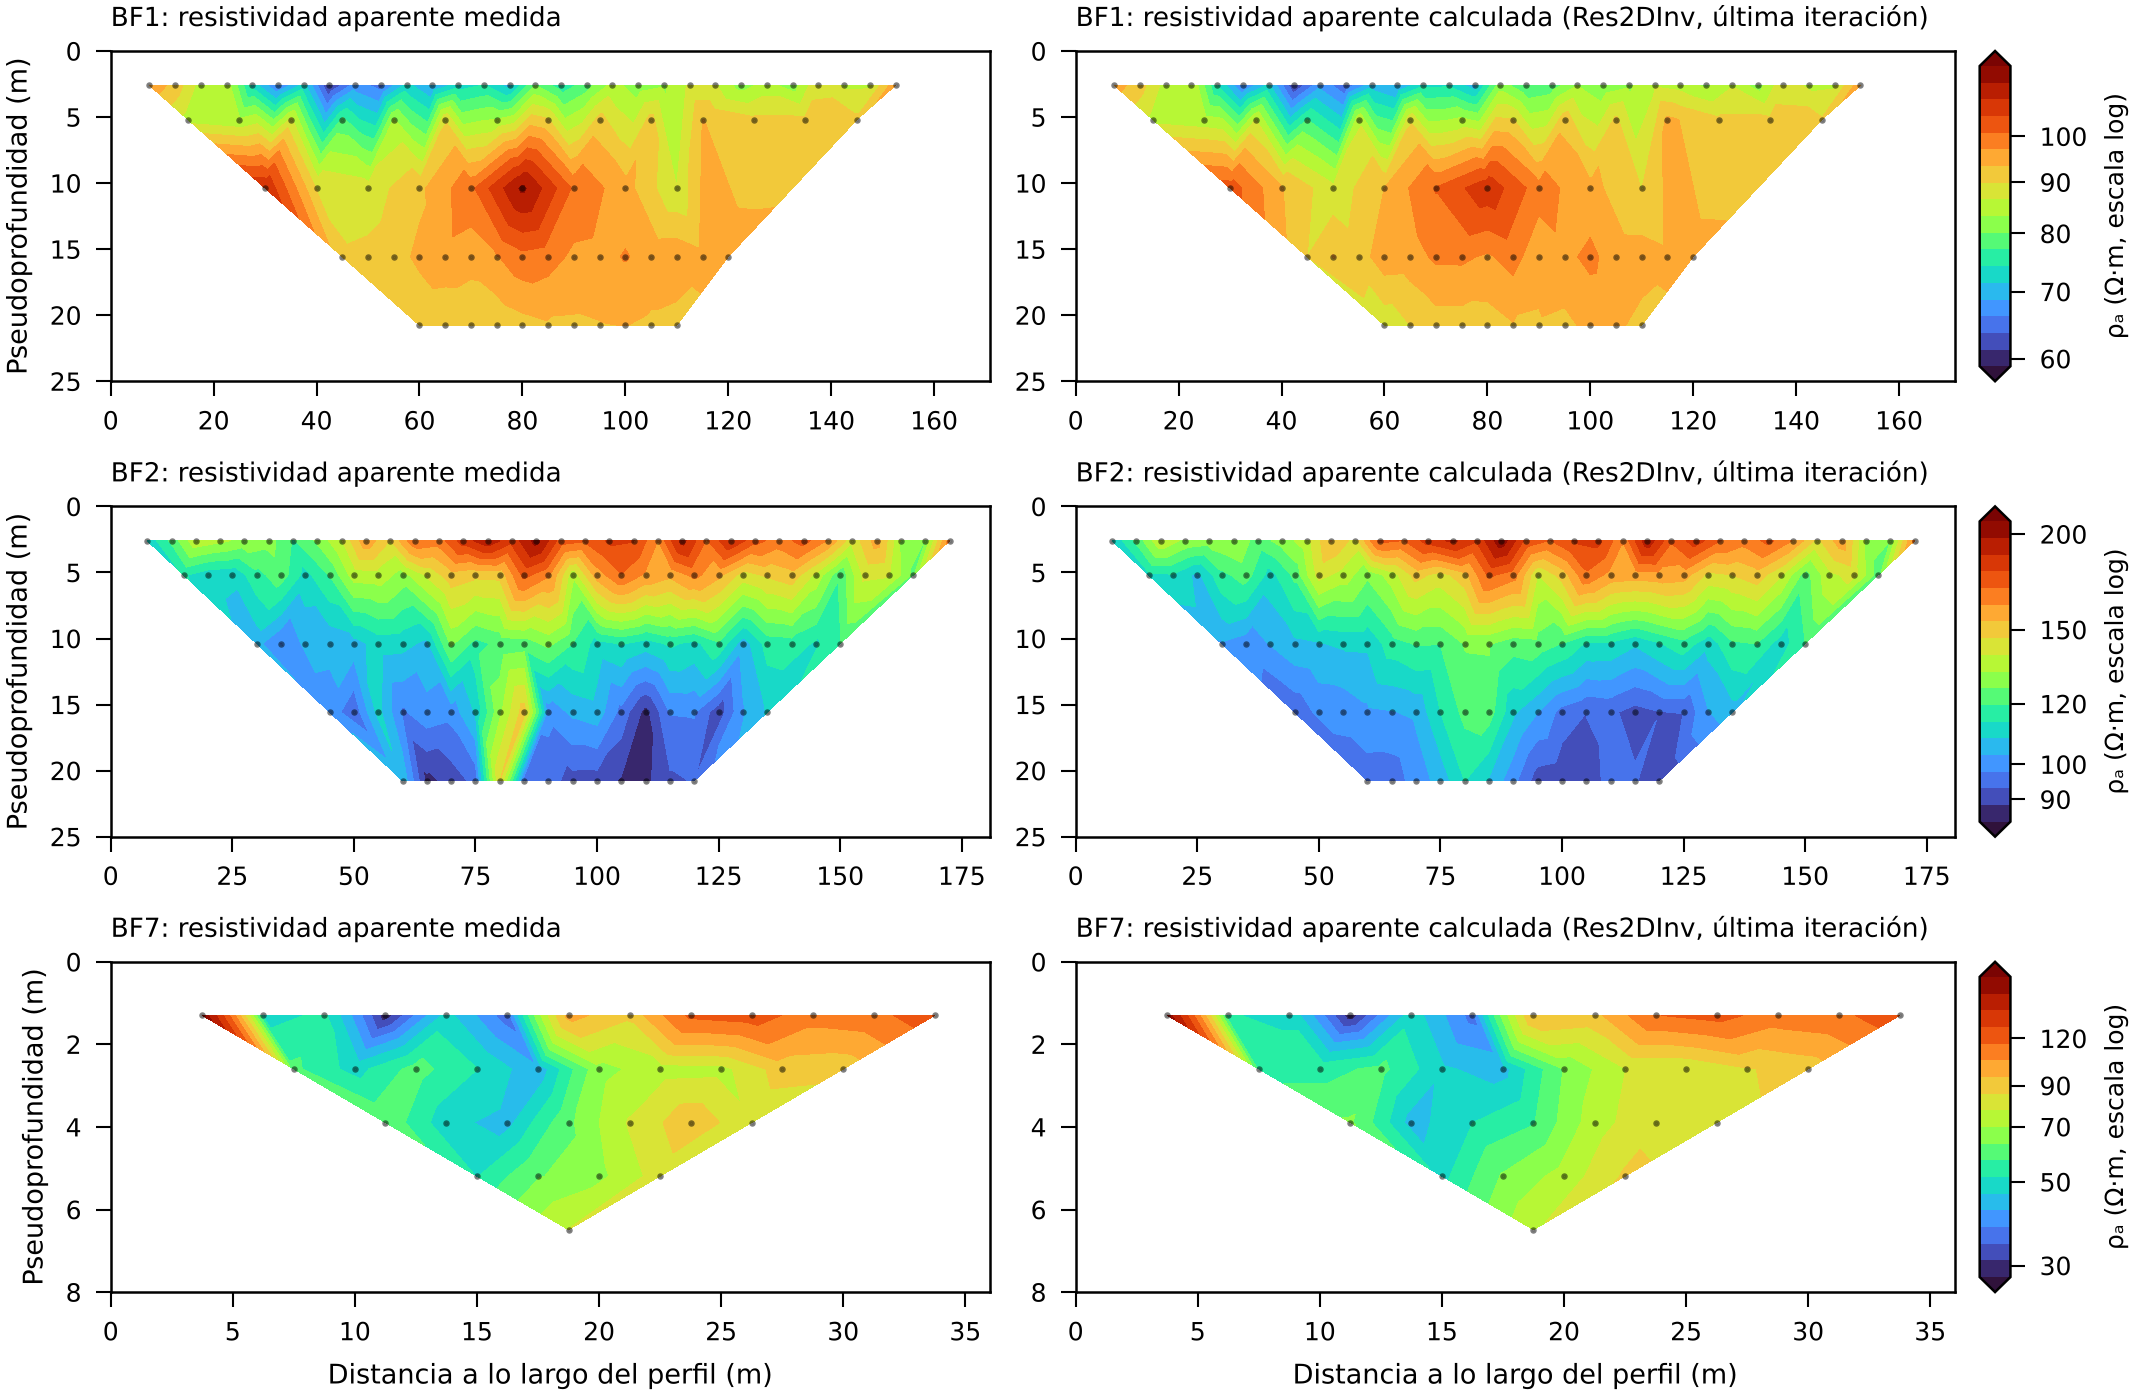
\includegraphics[width=0.62\textwidth]{f2_pseudosecciones.png}
\caption{Resistividad aparente medida (izquierda) y calculada por Res2DInv en la \'ultima iteraci\'on (derecha) para BF1, BF2 y BF7. Escala de color logar\'itmica en \ohmm, propia de cada perfil; los puntos son las mediciones.}
\label{fig:pseudo}
\end{figure*}

\subsection{Modelos invertidos}
La Fig.~\ref{fig:comp} (izquierda) presenta los modelos de Res2DInv con una escala com\'un de 10 a 1000\,\ohmm; la incertidumbre de cada bloque se resume en la Tabla~\ref{tab:conf}. BF1 es casi homog\'eneo: la mediana es 100\,\ohmm{} y el 55\,\% de los bloques est\'a entre 60 y 120\,\ohmm. BF2 tiene mediana de 145\,\ohmm{} y bloques de 23 a 640\,\ohmm, con una columna resistiva en $x\approx 93$--103\,m y varios bloques conductores a 8--14\,m de profundidad. BF7 llega a 11\,450\,\ohmm{} en un solo bloque, unas 68 veces la $\rho_a$ m\'axima medida (170\,\ohmm), sobre un cambio de pendiente. Ese valor parece un artefacto del modelo.


\subsection{Confiabilidad}
La Tabla~\ref{tab:conf} muestra por qu\'e el RMS no basta.
\begin{itemize}
\item \textbf{Un RMS bajo no garantiza contraste real.} BF1 tiene el menor RMS (1.64\,\%), pero sus datos casi no var\'ian. Su modelo (34--298\,\ohmm) tiene un rango mayor que los datos (61--114\,\ohmm). El RMS baj\'o de 4.6 a 1.64\,\% en 25 iteraciones y a\'un bajaba 0.97\,\% en la \'ultima. Mientras tanto, el contraste de la anomal\'ia H1 subi\'o de 1.1 a unas 2.7 veces el fondo.
\item \textbf{El error se concentra donde m\'as importa.} En BF2 el error crece con $a$: de 1.3\,\% con $a=5$\,m a 8\,\% con $a=40$\,m, y el 19\,\% de los datos pasa de 5\,\%. Los mayores desajustes est\'an en $x\approx 80$--85\,m y $z_p$ de 15 a 21\,m, donde la $\rho_a$ medida es 22 a 28\,\% mayor que la calculada. Ah\'i el art\'iculo marca una fractura. Un RMS de 4.9\,\% esconde que el modelo no reproduce esa se\~nal.
\item \textbf{La incertidumbre cambia mucho entre perfiles.} En BF1 es de 6\,\% en promedio y ning\'un bloque pasa de 15\,\%. En BF2 es de 19\,\% y el 77\,\% de los bloques pasa de 15\,\%. En BF7 es de 17\,\%. En BF2 y BF7 el valor llega al tope, cerca de 30\,\%. En BF1 y BF2 la sensibilidad mediana baja de unos 2.6 en la capa 1 a 0.2--0.5 en las capas 4 a 6.
\item \textbf{El modelo no es \'unico.} BF7 tiene m\'as bloques (49) que datos (35), y BF1 154 para 80; parte de la forma la decide el suavizado.
\item \textbf{Concordancia con el art\'iculo.} El RMS coincide en BF1 (1.6\,\%) y casi en BF2 (4.8 contra 4.92\,\%); en BF7 el art\'iculo da 3.3\,\% y el archivo 5.43\,\%. Puede ser otra corrida.
\end{itemize}

\begin{table}[!t]
\caption{Indicadores de confiabilidad de las inversiones de Res2DInv.}
\label{tab:conf}
\centering\footnotesize
\setlength{\tabcolsep}{3pt}
\begin{tabular}{p{3.55cm}ccc}
\toprule
Indicador & BF1 & BF2 & BF7 \\
\midrule
RMS inicial $\to$ final (\%) & 11.2 $\to$ 1.64 & 22.4 $\to$ 4.92 & 40.8 $\to$ 5.43 \\
RMS publicado en [1] (\%) & 1.6 & 4.8 & 3.3 \\
Iteraciones / cambio del RMS en la última (\%) & 25 / 0.97 & 16 / 0.38 & 24 / 0.07 \\
Error medio absoluto / máx. (\%) & 1.1 / 6 & 3.2 / 25 & 4.5 / 14 \\
Datos con error $>5$\,\% (\%) & 2 & 19 & 34 \\
Cociente $\rho_a$ máx./mín. & 1.9 & 2.3 & 5.9 \\
Datos / bloques & 80 / 154 & 122 / 180 & 35 / 49 \\
Sensibilidad media (mediana) & 1.01 (0.64) & 1.40 (0.66) & 1.28 (0.76) \\
Incertidumbre de bloque, media (\%) & 6 & 19 & 17 \\
Bloques con incert. $>15$\,\% (\%) & 0 & 77 & 57 \\
$\rho$ del modelo mín.--máx. (\ohmm) & 34--298 & 23--640 & 12--11450 \\
\bottomrule
\end{tabular}
\end{table}


\subsection{Inversi\'on propia y comparaci\'on con Res2DInv}
La Tabla~\ref{tab:perfiles} da los RMS. En BF1, BF2 y BF7 la inversi\'on propia llega a 2.61, 5.04 y 4.49\,\% (base), parecido a los 1.64, 4.92 y 5.43\,\% de Res2DInv. Los modelos propios son m\'as suaves: en BF1 van de 28 a 154\,\ohmm{} (Res2DInv, 34 a 298), que concuerda mejor con los datos (61 a 114\,\ohmm), y en BF7 de 19 a 528\,\ohmm, sin el bloque de 11\,450\,\ohmm. Eso apoya que ese valor sea un artefacto. De los siete perfiles sin modelo, BF3, BF8 y BF9 se ajustan bien (RMS 3.7 a 6.2\,\%). BF4, BF5, BF6 y BF10 no: el RMS base es de 7.9 a 13.8\,\% y entre 18 y 43\,\% de sus datos tiene error $>10$\,\%. Sus datos son ruidosos, con saltos entre puntos vecinos,. Estos perfiles no se interpretan.

La Fig.~\ref{fig:comp} compara los modelos de BF1, BF2 y BF7. De las 14 candidatas de BF1 y BF2, \textbf{3 se reproducen} (BF2-H1, H4 y L4), \textbf{5 en parte} (BF2-H3, H5, L1, L2 y L3) y \textbf{6 no} (BF1-H1, L1 y L2; BF2-H2, L5 y L6) (Tabla~\ref{tab:cand}, \'ultima columna). Las tres candidatas de BF1 no se reproducen (factor 1.07 a 1.17 con suavizado base): coincide con que sus datos casi no var\'ian y con que su contraste en Res2DInv crec\'ia con las iteraciones. Las que mejor resisten est\'an en BF2: BF2-H1 tiene factor 1.8 con suavizado base y 1.6 con el fuerte. En BF7 solo se reproduce L1; H1 y H3 salen con signo opuesto.

\begin{figure*}[!t]
\centering
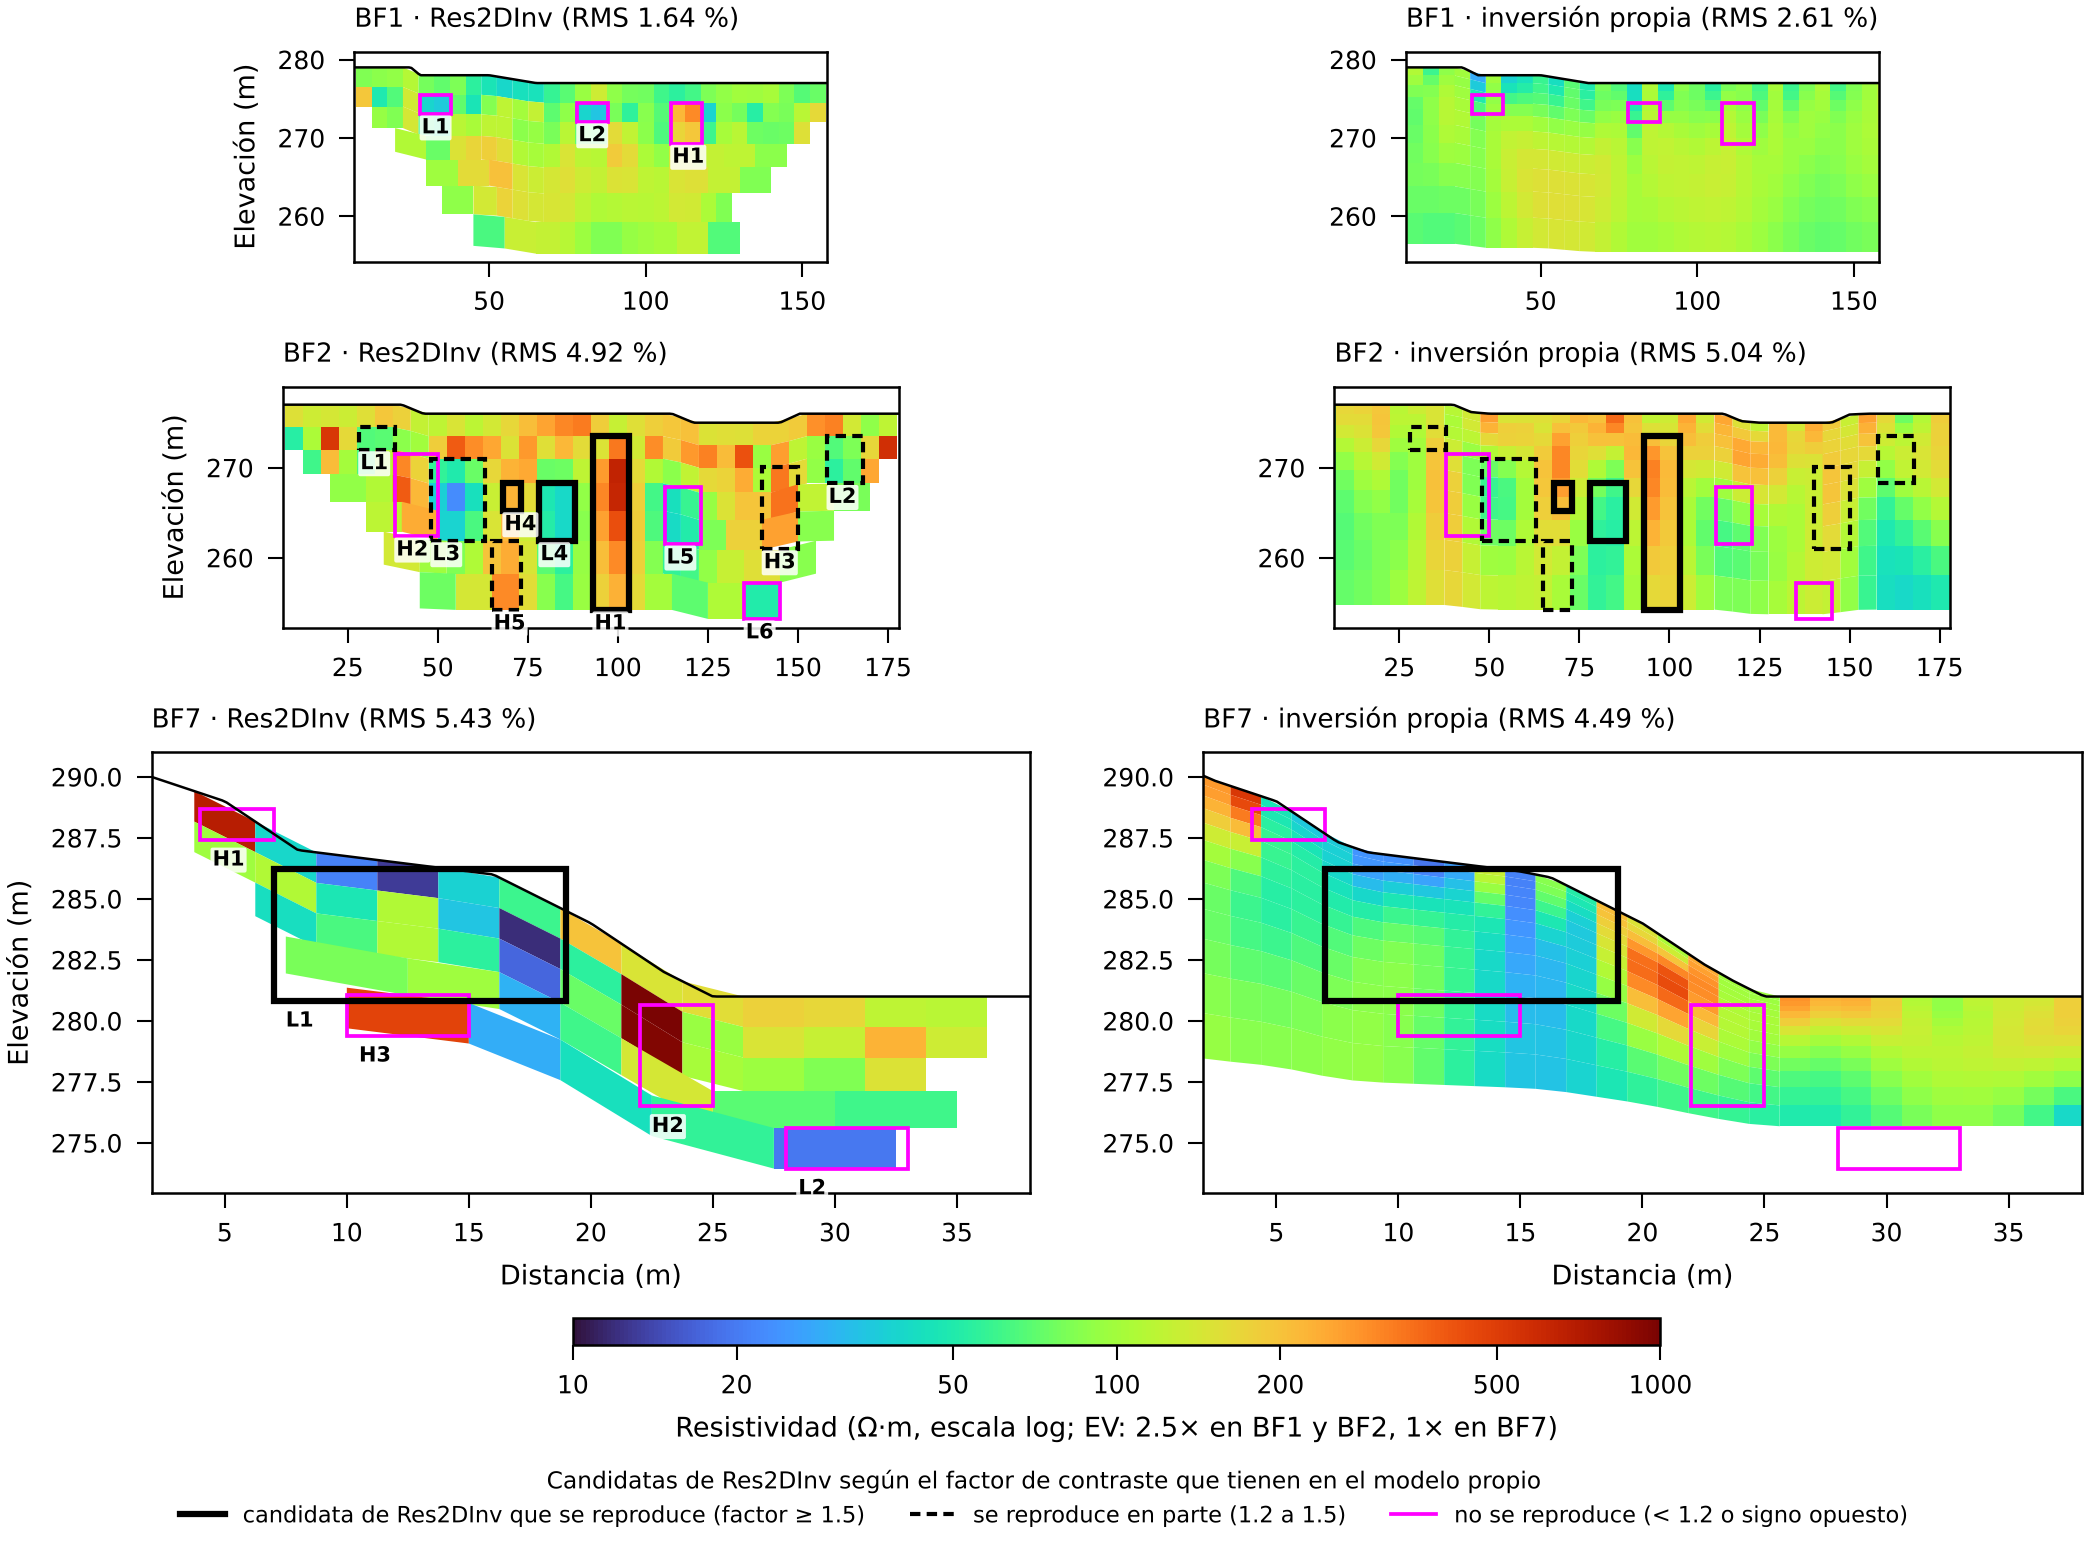
\includegraphics[width=0.72\textwidth]{f4_comparacion.png}
\caption{Modelos de Res2DInv (izquierda) e inversi\'on propia con suavizado base (derecha) para BF1, BF2 y BF7, con la misma escala de color. Los recuadros son las candidatas de Res2DInv, seg\'un si se reproducen en el modelo propio (Tabla~\ref{tab:cand}).}
\label{fig:comp}
\end{figure*}

La Fig.~\ref{fig:propios} muestra los modelos propios de los otros siete perfiles. Con el criterio de arriba hay 70 candidatas en los diez perfiles; 50 est\'an en los cuatro perfiles de ajuste pobre y se descartan, y de las 20 restantes, 18 no est\'an limitadas a la primera capa. Seis son prioritarias (Tabla~\ref{tab:prop}). BF2-pH3 y BF7-pL1 coinciden con BF2-H1 y BF7-L1 de Res2DInv. Las otras cuatro son nuevas. BF3-pL1, de 7\,\ohmm{} contra 21 de fondo, es muy conductora y superficial (0 a 5\,m) y puede ser arcilla, sal o humedad. BF3-pH2, BF8-pL3 y BF9-pL1 est\'an a 3 a 14\,m de profundidad. Con 35 datos y ladera, BF7-pL1 no se debe leer m\'as all\'a de lo que dicen los datos.

\begin{figure*}[!t]
\centering
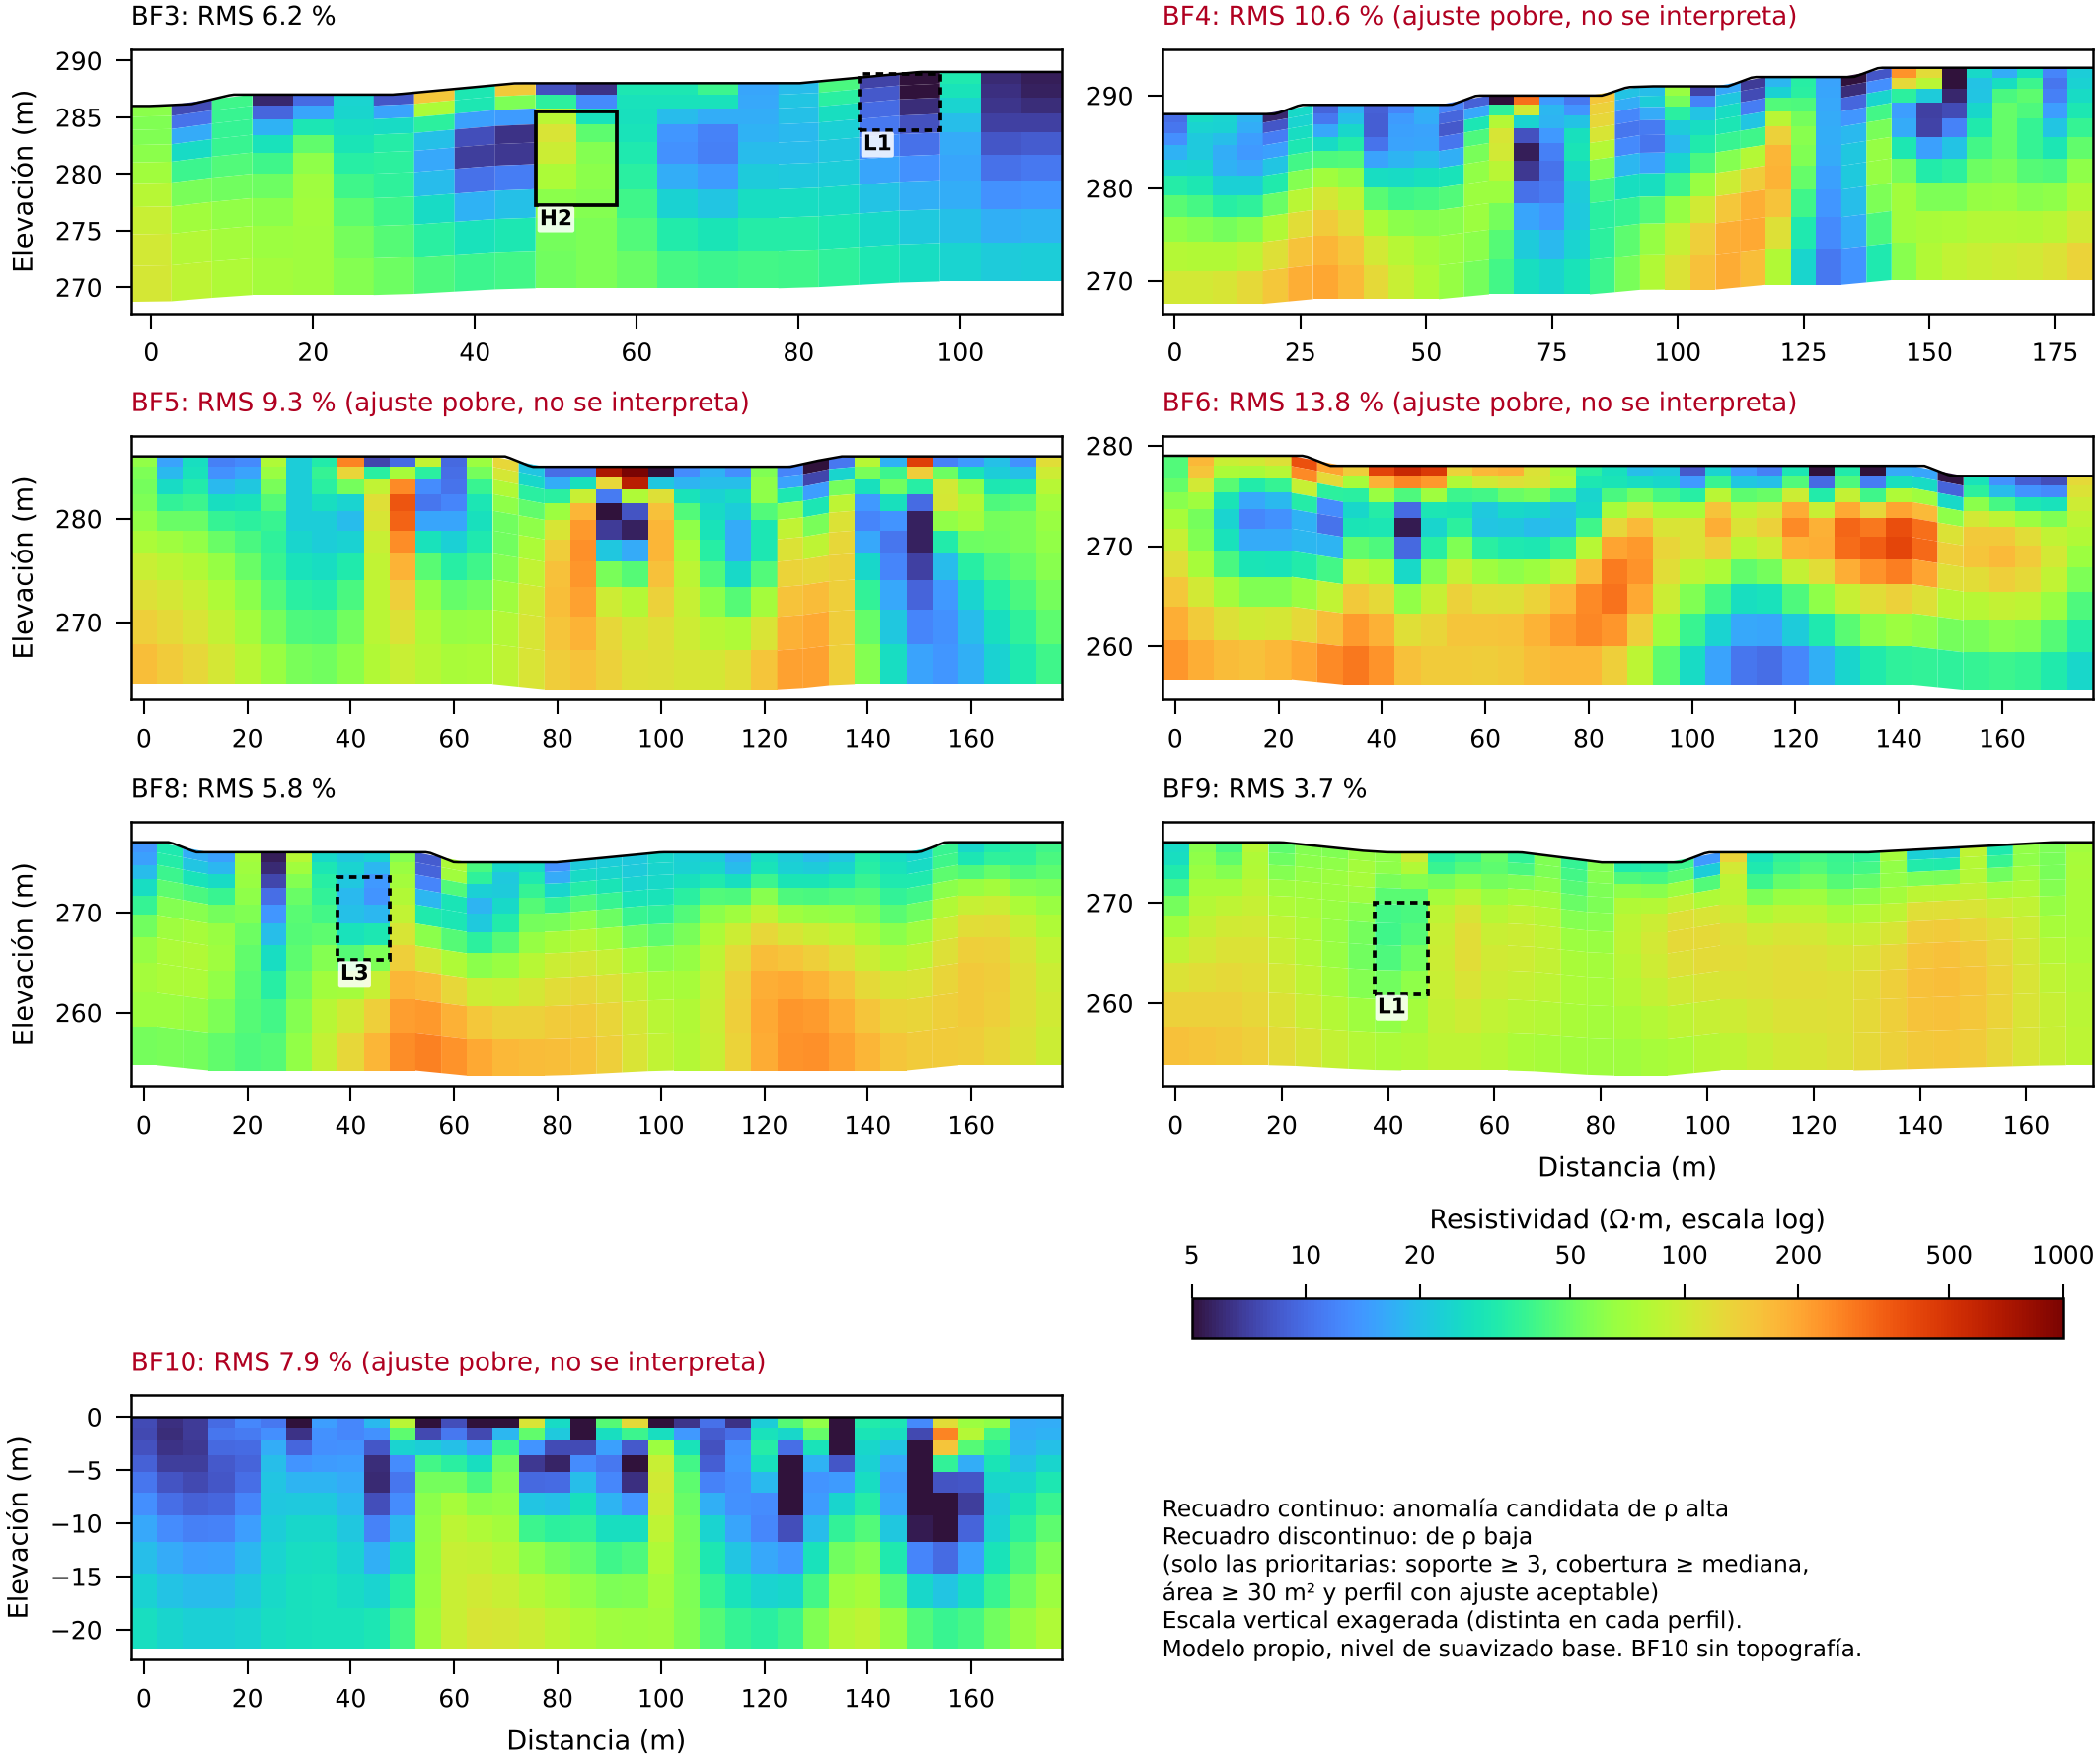
\includegraphics[width=0.66\textwidth]{f5_modelos_propios.png}
\caption{Inversi\'on propia (suavizado base) de los siete perfiles sin modelo de Res2DInv, con la misma escala logar\'itmica (\ohmm). Los t\'itulos en rojo son perfiles con ajuste pobre. Los recuadros son las candidatas prioritarias: continuo, $\rho$ alta; discontinuo, $\rho$ baja.}
\label{fig:propios}
\end{figure*}

\begin{table}[!t]
\caption{Candidatas prioritarias del modelo propio (prefijo p). BF2-pH3 coincide con BF2-H1 de Res2DInv y BF7-pL1 con BF7-L1. Columnas como en la Tabla~\ref{tab:cand}; $C$ es el contraste con el fondo.}
\label{tab:prop}
\centering\footnotesize
\setlength{\tabcolsep}{2.6pt}
\begin{tabular}{lccccccc}
\toprule
ID & $x$ (m) & E (m) & N (m) & $z$ (m) & $\rho$/fondo & $C$ & $S$ \\
\midrule
BF2-pH3 & 97 & 651815 & 3622137 & 5.0--17.8 & 224/97 & 2.3 & 3 \\
BF3-pH2 & 52 & 651972 & 3621736 & 2.5--10.8 & 73/22 & 3.4 & 3 \\
BF3-pL1 & 92 & 651969 & 3621695 & 0.0--5.0 & 7/21 & 0.3 & 4 \\
BF7-pL1 & 13 & 651955 & 3622430 & 0.0--7.1 & 36/102 & 0.4 & 4 \\
BF8-pL3 & 42 & 652072 & 3622549 & 2.5--10.8 & 22/55 & 0.4 & 3 \\
BF9-pL1 & 41 & 651662 & 3622525 & 5.0--14.1 & 45/98 & 0.5 & 3 \\
\bottomrule
\end{tabular}
\end{table}

\subsection{Anomal\'ias candidatas}
La Tabla~\ref{tab:cand} lista las 14 anomal\'ias de BF1 y BF2 con su posici\'on UTM aproximada. De BF7 salieron cinco regiones, pero se descartan por no ser concluyentes: el perfil est\'a en una ladera de unos 18°, tiene 35 datos para 49 bloques y los bloques m\'as extremos tienen incertidumbre de 29 a 30\,\%. Las dem\'as se agrupan en tres tipos:
\begin{itemize}
\item \textbf{Resistividad alta cerrada (H1--H5 en BF2; H1 en BF1).} Pueden ser un hueco con aire, pero tambi\'en roca cementada o material seco. BF2-H1 es la mayor (columna de 19\,m, 344\,\ohmm{} contra 117\,\ohmm{} de fondo). Su contraste ya era 1.9 en la iteraci\'on 4 y se estabiliza cerca de 3. En cambio, BF1-H1 pasa de 1.3 a 2.7 veces el fondo entre la iteraci\'on 4 y la 25, as\'i que su amplitud depende del suavizado. BF2-H2 y BF2-H3 tienen $S=1$. En la inversi\'on propia, BF2-H1 y BF2-H4 se reproducen (factor 1.8 y 2.0), BF2-H3 en parte y BF2-H2 no; BF1-H1 no se reproduce (1.08), as\'i que su amplitud parece un efecto del suavizado.
\item \textbf{Resistividad baja cerrada (L3--L5 en BF2; L1--L2 en BF1).} A 8--14\,m en BF2 (40--46\,\ohmm{} contra 115--117\,\ohmm) pueden ser lentes de arcilla, arena h\'umeda o huecos rellenos de material conductor. El art\'iculo describe huecos rellenos o semirrellenos y marca en BF2 una cavidad con relleno conductor hacia $x\approx 55$--60\,m (le\'ido de la figura), que coincide con BF2-L3 \cite{melouah2016}. BF2-L3 solo se reproduce en parte (factor 1.26) y BF2-L4 s\'i (1.54); BF2-L5 y BF2-L6 no. Los bloques bajos de 2.5 a 5\,m en $x\approx 33$\,m (BF1-L1 y BF2-L1, $S=4$) son superficiales y est\'an junto a un cambio de pendiente. Conviene revisarlos antes de darles un significado geol\'ogico.
\item \textbf{Zona de contraste lateral en BF2, $x\approx 80$--103\,m.} Aqu\'i coinciden el desajuste del modelo en $x\approx 80$--85\,m, la columna H1 y el bloque bajo L4 en $x\approx 78$--88\,m. Un contraste vertical as\'i puede deberse a una fractura o falla, que el art\'iculo marca en esa zona. Con la inversi\'on propia, H1 y L4 se mantienen, lo que refuerza esta zona.
\end{itemize}
Un bloque aislado de 524\,\ohmm{} a 2.5--5\,m en $x=20$\,m de BF2 coincide con la ``cavidad'' superficial del art\'iculo, pero queda bajo el \'area m\'inima (unos 12\,m$^2$). En general, los datos medidos en la zona de las candidatas valen solo 0.8 a 1.2 veces la mediana de su nivel, mucho menos que el contraste de 2 a 3 del modelo. Por eso, la posici\'on y el signo de las anomal\'ias son m\'as confiables que su amplitud. Las prioritarias de los otros perfiles est\'an en la Tabla~\ref{tab:prop}.

\begin{table*}[!t]
\caption{Anomal\'ias candidatas en BF1 y BF2. $x$: distancia sobre el perfil; E, N: UTM 31N aproximados (error de 3 a 10\,m); $z$: intervalo de profundidad; $\rho$/fondo: resistividad media de la anomal\'ia y mediana de su capa (\ohmm); $C$: contraste final (entre par\'entesis, en la iteraci\'on 4); $U$: incertidumbre media (\%); $S$: \'indice de soporte 0--4. Factor propio: factor de contraste con signo en la inversi\'on propia (suavizado d\'ebil / base / fuerte) sobre el mismo recuadro. Rep.: se reproduce ($\ge1.5$ con suavizado base), en parte (1.2 a 1.5) o no. Ninguna fila es una cavidad comprobada.}
\label{tab:cand}
\centering\footnotesize
\setlength{\tabcolsep}{4.5pt}
\begin{tabular}{lcccccccccc}
\toprule
ID & $x$ (m) & E (m) & N (m) & $z$ (m) & $\rho$/fondo & $C$ ($C_{4}$) & $U$ (\%) & $S$ & Factor propio & Rep. \\
\midrule
BF1-H1 & 114 & 651840 & 3622287 & 2.5--7.8 & 231/84 & 2.7 (1.3) & 7 & 2 & 1.10 / 1.08 / 1.08 & no \\
BF1-L1 & 33 & 651849 & 3622365 & 2.5--5.0 & 38/80 & 0.5 (0.7) & 6 & 4 & 1.30 / 1.17 / 1.15 & no \\
BF1-L2 & 83 & 651844 & 3622317 & 2.5--5.0 & 37/80 & 0.5 (0.8) & 5 & 2 & 1.09 / 1.07 / 1.04 & no \\
BF2-H1 & 99 & 651815 & 3622135 & 2.5--21.8 & 344/117 & 2.9 (1.9) & 25 & 2 & 1.83 / 1.82 / 1.61 & sí \\
BF2-H2 & 43 & 651825 & 3622190 & 5.0--14.1 & 284/118 & 2.4 (1.1) & 23 & 1 & 1.06 / 0.97 / 0.92 & no \\
BF2-H3 & 146 & 651806 & 3622088 & 5.0--14.1 & 295/117 & 2.5 (1.2) & 23 & 1 & 1.76 / 1.46 / 1.27 & parcial \\
BF2-H4 & 70 & 651820 & 3622163 & 7.8--10.8 & 226/110 & 2.1 (1.3) & 26 & 2 & 2.74 / 1.98 / 1.49 & sí \\
BF2-H5 & 70 & 651820 & 3622164 & 14.1--21.8 & 274/104 & 2.6 (1.4) & 20 & 2 & 1.70 / 1.28 / 1.14 & parcial \\
BF2-L1 & 33 & 651827 & 3622200 & 2.5--5.0 & 68/165 & 0.4 (0.6) & 18 & 4 & 1.36 / 1.26 / 1.21 & parcial \\
BF2-L2 & 162 & 651803 & 3622072 & 2.5--7.8 & 66/148 & 0.4 (0.8) & 21 & 2 & 1.12 / 1.30 / 1.36 & parcial \\
BF2-L3 & 54 & 651823 & 3622179 & 5.0--14.1 & 40/116 & 0.3 (0.7) & 23 & 2 & 1.42 / 1.26 / 1.19 & parcial \\
BF2-L4 & 83 & 651818 & 3622150 & 7.8--14.1 & 45/115 & 0.4 (0.8) & 26 & 1 & 2.21 / 1.54 / 1.25 & sí \\
BF2-L5 & 117 & 651812 & 3622116 & 7.8--14.1 & 46/117 & 0.4 (0.6) & 26 & 2 & 1.36 / 1.16 / 1.09 & no \\
BF2-L6 & 140 & 651807 & 3622094 & 17.8--21.8 & 50/101 & 0.5 (0.6) & 5 & 3 & 0.60 / 0.74 / 0.90 & no \\
\bottomrule
\end{tabular}
\end{table*}

\begin{figure*}[!t]
\centering
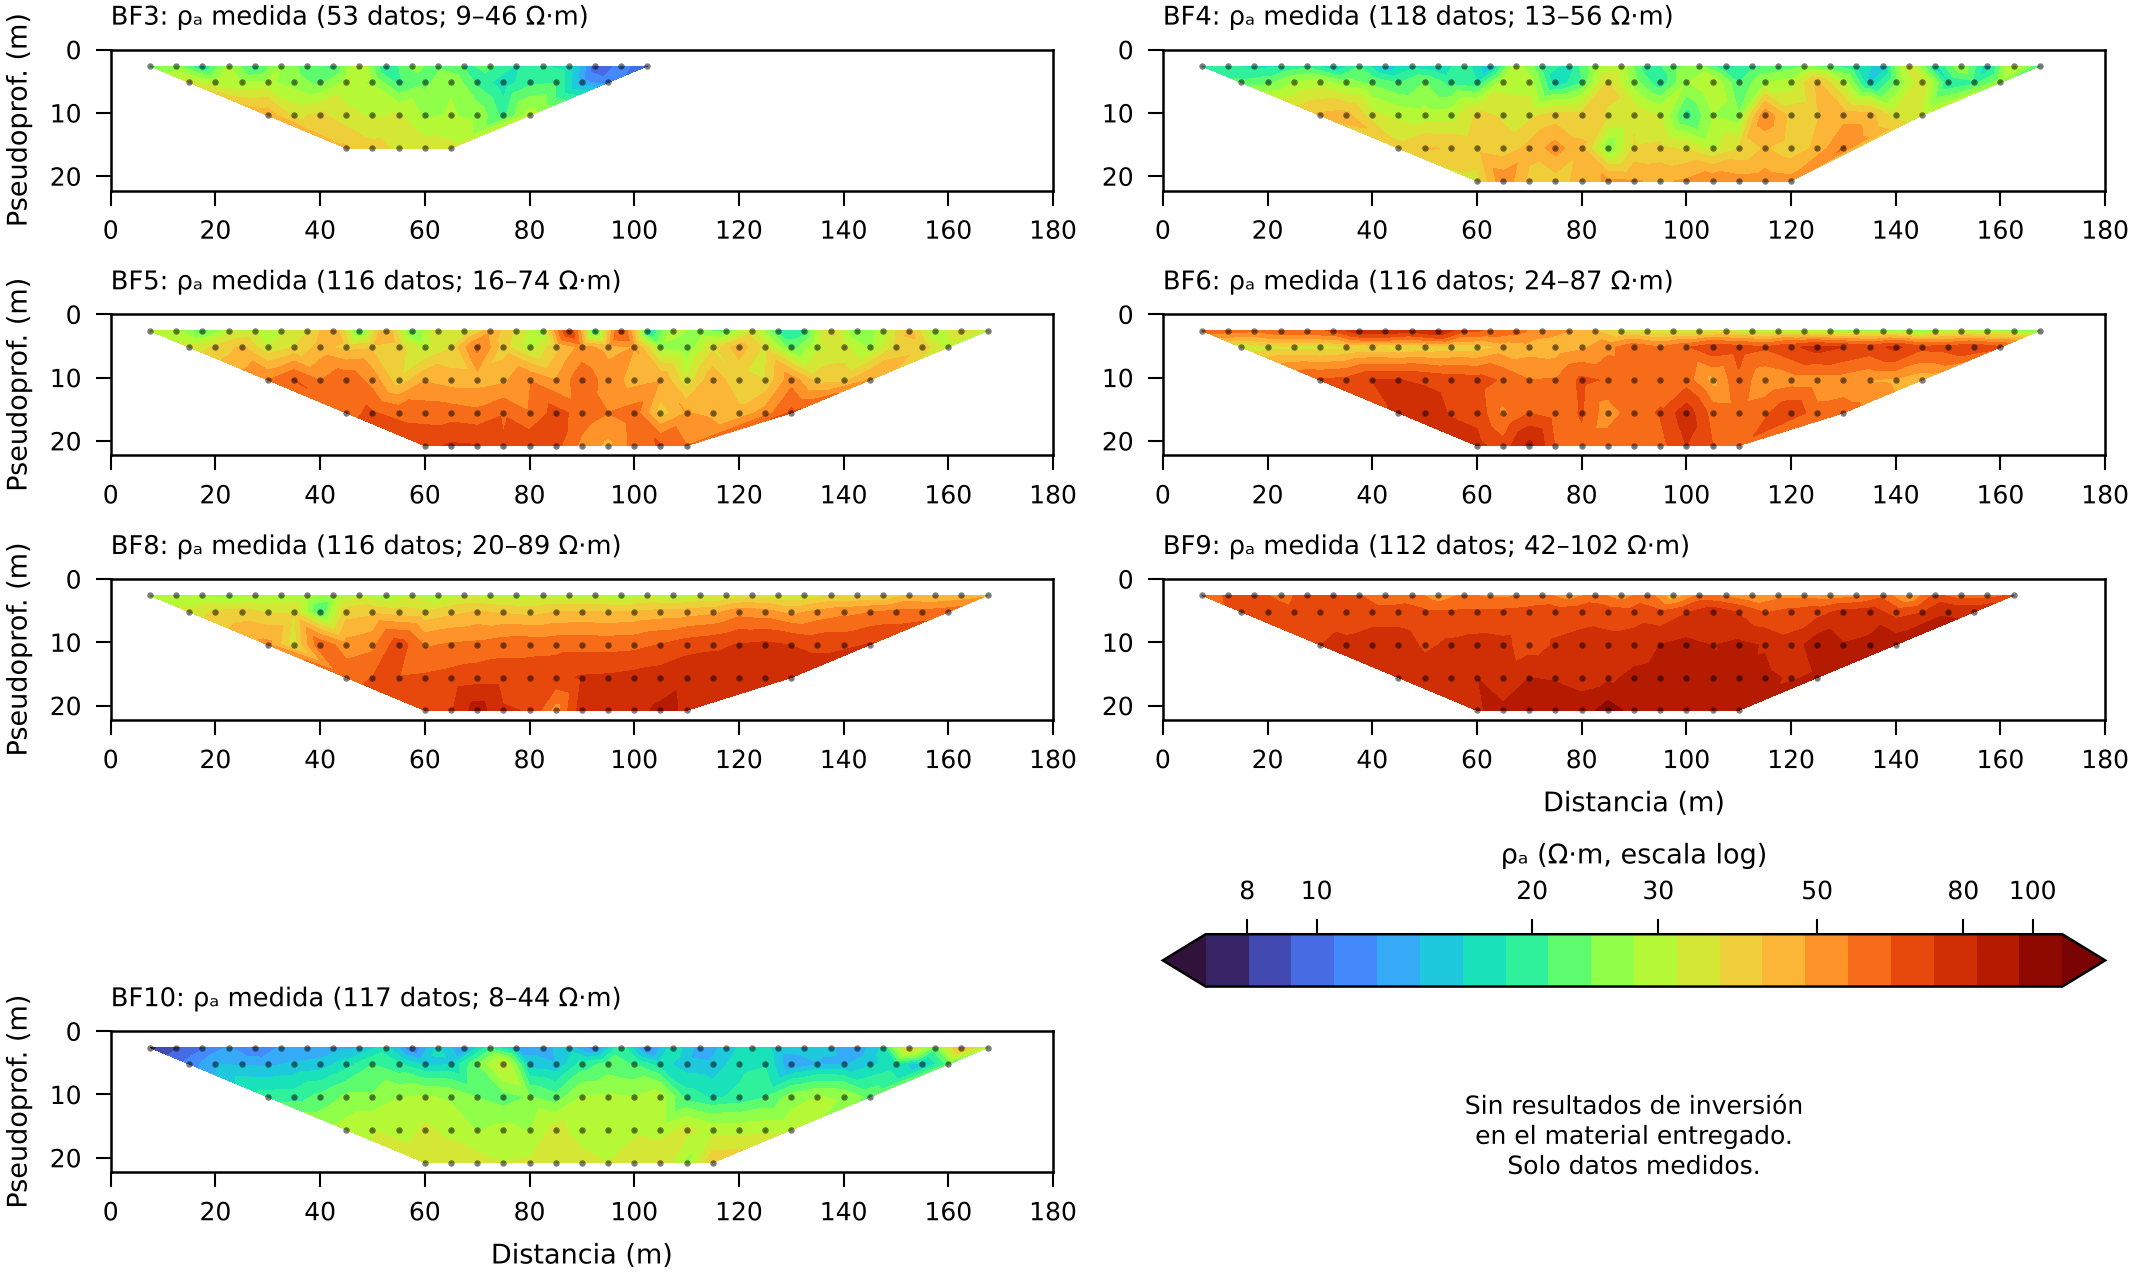
\includegraphics[width=0.62\textwidth]{f5_otros_perfiles.png}
\caption{Resistividad aparente medida en los siete perfiles sin modelo de Res2DInv (BF3 a BF6, BF8 a BF10), con la misma escala de color logar\'itmica (\ohmm).}
\label{fig:otros}
\end{figure*}

\subsection{Orientaci\'on de los perfiles}
Las fracturas del art\'iculo tienen direcciones N\,50--70° y N\,150--170°. BF1 y BF2 (casi norte--sur, N\,6° y N\,10°) cruzan el primer conjunto con 40° a 64° y el segundo con 16° a 40°. BF6, BF7 y BF8 (N\,63° a N\,80°) son casi paralelos al primer conjunto, y BF4, BF5 y BF9, al segundo. Una estructura paralela al perfil se ve mal en 2D, as\'i que no ver anomal\'ia en esos perfiles no descarta fracturas. Una versi\'on de congreso del mismo grupo da N\,30--60° y N\,140--160° \cite{melouah2013}; la conclusi\'on no cambia.

\section{Modelo conceptual}
La Fig.~\ref{fig:concept} junta los datos con el art\'iculo y con la geolog\'ia de la Fig.~\ref{fig:geo}. Es una hip\'otesis: no se conoce la forma de las unidades por debajo de unos 8\,m ni la profundidad de la caliza. Seg\'un el art\'iculo, las fracturas abren caminos para el agua de lluvia, que con CO$_2$ y \'acido h\'umico disuelve carbonatos y yeso. As\'i se forman huecos de tama\~no m\'etrico en un aluvi\'on blando (19\,bar), con arenisca debajo, que los sedimentos rellenan en parte \cite{melouah2016}. Con este esquema, las candidatas H se explican como huecos, roca compacta o material seco, y las L como relleno h\'umedo o de arcilla. La ERT con $a\le 40$\,m solo llega a unos 22\,m, as\'i que no dice nada de la caliza ni de huecos m\'as profundos.

\begin{figure*}[!t]
\centering
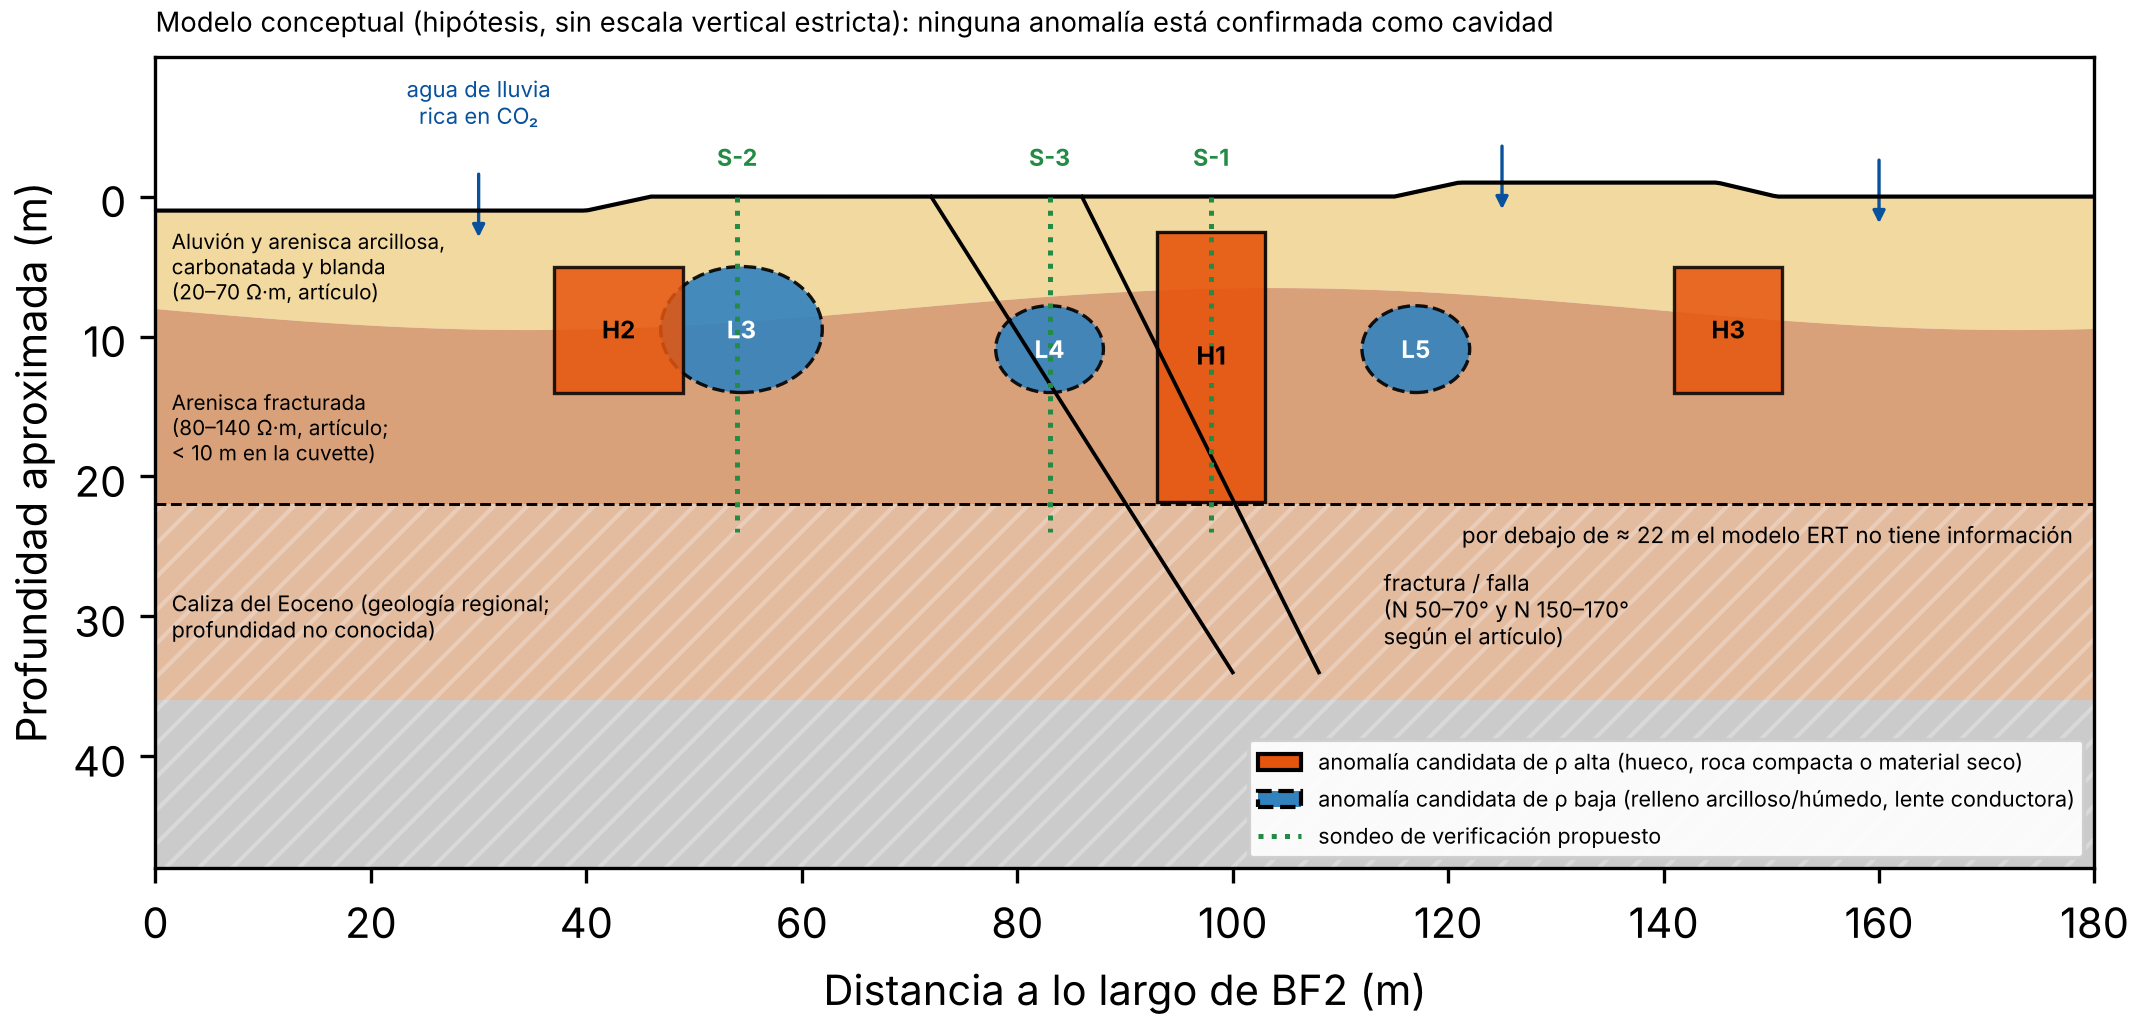
\includegraphics[width=0.68\textwidth]{f6_conceptual.png}
\caption{Modelo conceptual a lo largo de BF2 (hip\'otesis). Las anomal\'ias tienen la posici\'on y profundidad de la Tabla~\ref{tab:cand}; los sondeos S-1 a S-3 son propuestas de verificaci\'on (Tabla~\ref{tab:verif}).}
\label{fig:concept}
\end{figure*}

\section{Informaci\'on adicional y verificaci\'on}
Para pasar de ``compatible con'' a ``confirmado'' hay que saber si existe un hueco, su tama\~no, el espesor de su techo, si est\'a conectado y por d\'onde entra el agua. La Tabla~\ref{tab:verif} propone las acciones, en orden de prioridad. Los primeros sondeos deben ir en las candidatas que se reproducen en ambos modelos (BF2-H1, BF2-L4) y en BF2-L3, que coincide con el art\'iculo; despu\'es, en las prioritarias nuevas (Tabla~\ref{tab:prop}).

\begin{table*}[!t]
\caption{Acciones de verificaci\'on propuestas.}
\label{tab:verif}
\centering\footnotesize
\renewcommand{\arraystretch}{1.1}
\begin{tabular}{p{0.3\textwidth}p{0.36\textwidth}p{0.24\textwidth}}
\toprule
Acci\'on & Qu\'e resuelve & D\'onde \\
\midrule
Sondeos con n\'ucleo y registro de p\'erdida de lodo o ca\'ida de la barra & Distinguen hueco vac\'io, hueco relleno, roca compacta y lente de arcilla; miden el espesor del techo & S-1 (BF2-H1), S-2 (L3), S-3 (L4); luego BF3-pH2, BF8-pL3, BF9-pL1 \\
Georradar de 100 y 200\,MHz sobre los mismos perfiles & Detecta huecos poco profundos ($<5$\,m) que la ERT no resuelve & BF1 y BF2 completos, BF1-L1/BF2-L1 \\
Microgravimetr\'ia & Un hueco vac\'io resta densidad, sin importar la resistividad & L\'inea BF1+BF2, paso de 2.5--5\,m \\
ERT nueva con otro arreglo y paso de 2.5\,m; perfiles cruzados y malla 3D & Reduce la ambig\"uedad del 2D y detecta fracturas paralelas a los perfiles & Cruz sobre BF2 en $x\approx 90$\,m; perfiles N\,--\,S en BF6--BF8 \\
Prueba sint\'etica con el mismo arreglo (modelo directo de huecos de 3 a 10\,m) & Dice si un hueco de ese tama\~no y profundidad se ver\'ia, y con qu\'e contraste & Geometr\'ia de BF1 y BF2 \\
Inversi\'on de los siete perfiles sin modelo de Res2DInv con ese programa y con datos depurados; \'indice de profundidad de investigaci\'on \cite{oldenburg1999} & Contrasta los resultados entre programas y fija la zona bien resuelta & Los diez perfiles \\
Revisi\'on del campo y repetici\'on de la medida (contacto de electrodos, ruido) & Los datos de BF4, BF5, BF6 y BF10 son ruidosos y no permiten interpretar & Esos cuatro perfiles \\
Muestras de suelo y roca (yeso, carbonatos, humedad, grano, resistividad en laboratorio) y revisi\'on de afloramientos y rumbos de fractura & Indican qu\'e material da 40, 100 o 300\,\ohmm{} y confirman unidades y fracturas, que aqu\'i vienen de un mapa regional & Columnas de los sondeos; alrededor de la depresi\'on y de BF1--BF2 \\
Nivel fre\'atico, calidad del agua, trazadores, nivelaci\'on y monitoreo de hundimientos & Eval\'uan el agua que se pierde, el riesgo para el acu\'ifero y la deformaci\'on del terreno & Pozos cercanos, puntos de infiltraci\'on y alrededor de BF2 \\
\bottomrule
\end{tabular}
\end{table*}

\section{Limitaciones}
(i) La inversi\'on propia puede diferir de la de Res2DInv (otra malla, error supuesto de 3\,\%, sin edici\'on de datos), y los modelos de BF1, BF2 y BF7 de Res2DInv no se recalcularon. Las candidatas de los siete perfiles restantes dependen solo de la inversi\'on propia. (ii) El modelo es 2D y el terreno no lo es; estructuras distintas pueden dar la misma respuesta y el suavizado cambia las formas. (iii) La incertidumbre de Res2DInv tiene un tope de 30\,\%; el $S$ propio no tiene incertidumbre por bloque. (iv) Los umbrales de $|\Delta|$, de $S$, del ajuste aceptable y del factor de reproducci\'on son de este trabajo. (v) BF4, BF5, BF6 y BF10 tienen datos ruidosos y no se interpretan; quiz\'a con edici\'on de datos se podr\'ian usar. (vi) Las coordenadas tienen precisi\'on de unos 3\,m. (vii) BF7 est\'a en una ladera y tiene pocos datos, y su \texttt{.INV} puede no ser la corrida del art\'iculo. (viii) No se dispone de datos de georradar, sondeos ni muestras, y la elevaci\'on no tiene referencia absoluta. (ix) La geolog\'ia viene de un mapa regional y del texto del art\'iculo, con error de unos 100\,m en el mapa. (x) La imagen satelital de la Fig.~\ref{fig:mapa} se ubic\'o con un solo punto y la barra de escala (unos 15\,m de error); se desconocen su fecha y su resoluci\'on original. La estructura circular cerca de BF7 no se interpreta.

\section{Conclusiones}
\begin{enumerate}
\item Se ubicaron los diez perfiles en UTM 31N (coincidencia de 0.0005\,m con la hoja de c\'alculo) y sobre una imagen satelital. Se dibujaron pseudosecciones y modelos de los diez, con escala y unidades: BF1, BF2 y BF7 con Res2DInv y con la inversi\'on propia, y los otros siete con esta \'ultima.
\item El RMS (1.64, 4.92 y 5.43\,\% en Res2DInv) no basta. BF1 se ajusta bien porque casi no tiene contraste, y ninguna de sus tres candidatas se reproduce en la inversi\'on propia. BF2 tiene 77\,\% de bloques con incertidumbre mayor a 15\,\%. El bloque de 11\,450\,\ohmm{} de BF7 es un artefacto.
\item De las 14 candidatas de BF1 y BF2, 3 se reproducen (BF2-H1, H4 y L4), 5 en parte y 6 no. La zona de BF2 en $x\approx 80$--103\,m es la m\'as robusta y puede ser una fractura. Ninguna est\'a comprobada como cavidad.
\item BF4, BF5, BF6 y BF10 no se pudieron interpretar por sus datos ruidosos. En los otros perfiles hay seis candidatas prioritarias (BF2-pH3, BF3-pH2, BF3-pL1, BF7-pL1, BF8-pL3 y BF9-pL1). Las de resistividad alta pueden ser huecos, roca compacta o material seco; las de baja, relleno h\'umedo, arcilla o sal.
\item La posici\'on y el signo de las anomal\'ias son m\'as confiables que su amplitud. Las que m\'as conviene verificar primero son BF2-H1, BF2-L4 y BF2-L3.
\item El modelo conceptual (fracturas, disoluci\'on y relleno parcial) es una hip\'otesis: la ERT llega a unos 22\,m.
\item Para evaluar la importancia ambiental y geot\'ecnica hacen falta sondeos, georradar, microgravimetr\'ia, ERT cruzada o 3D, pruebas sint\'eticas, la inversi\'on de todos los perfiles con Res2DInv y datos de agua y de resistencia del terreno (Tabla~\ref{tab:verif}).
\end{enumerate}

\begin{thebibliography}{00}
\bibitem{melouah2016} O. Melouah y A. Zeddouri, ``Use of geophysical methods for the demonstration of karstic phenomena in southern Algeria: Guerrara area (district of Gharda\"ia, Algeria),'' \textit{J. Fundam. Appl. Sci.}, vol. 8, n.\textsuperscript{o} 3, pp. 1097--1114, 2016.
\bibitem{coskun2012} N. Coskun, ``The effectiveness of electrical resistivity imaging in sinkhole investigations,'' \textit{Int. J. Phys. Sci.}, vol. 7, n.\textsuperscript{o} 15, pp. 2398--2405, 2012.
\bibitem{elkhammari2007} K. El Khammari \textit{et al.}, ``Imagerie combin\'ee g\'eo\'electrique--radar g\'eologique des cavit\'es souterraines de la ville de Zaouit Ech Cheikh (Maroc),'' \textit{C. R. G\'eosci.}, vol. 339, n.\textsuperscript{o} 7, pp. 460--467, 2007.
\bibitem{loke1996} M. H. Loke y R. D. Barker, ``Rapid least-squares inversion of apparent resistivity pseudosections using a quasi-Newton method,'' \textit{Geophys. Prospect.}, vol. 44, n.\textsuperscript{o} 1, pp. 131--152, 1996.
\bibitem{edwards1977} L. S. Edwards, ``A modified pseudosection for resistivity and IP,'' \textit{Geophysics}, vol. 42, n.\textsuperscript{o} 5, pp. 1020--1036, 1977.
\bibitem{melouah2013} O. Melouah, A. Zeddouri y H. Laouini, ``\'Etude de la zone d'infiltration des aquif\`eres karstiques par m\'ethodes g\'eophysiques (cas de la r\'egion de Gu\'errara, Gharda\"ia),'' en \textit{S\'eminaire SIHE}, Univ. Kasdi Merbah Ouargla, 2013.
\bibitem{oldenburg1999} D. W. Oldenburg y Y. Li, ``Estimating depth of investigation in DC resistivity and IP surveys,'' \textit{Geophysics}, vol. 64, n.\textsuperscript{o} 2, pp. 403--416, 1999.
\end{thebibliography}
\end{document}
